\begin{figure}[!htb]
\centering
\begin{subfigure}[t]{0.48\linewidth}
  \centering
  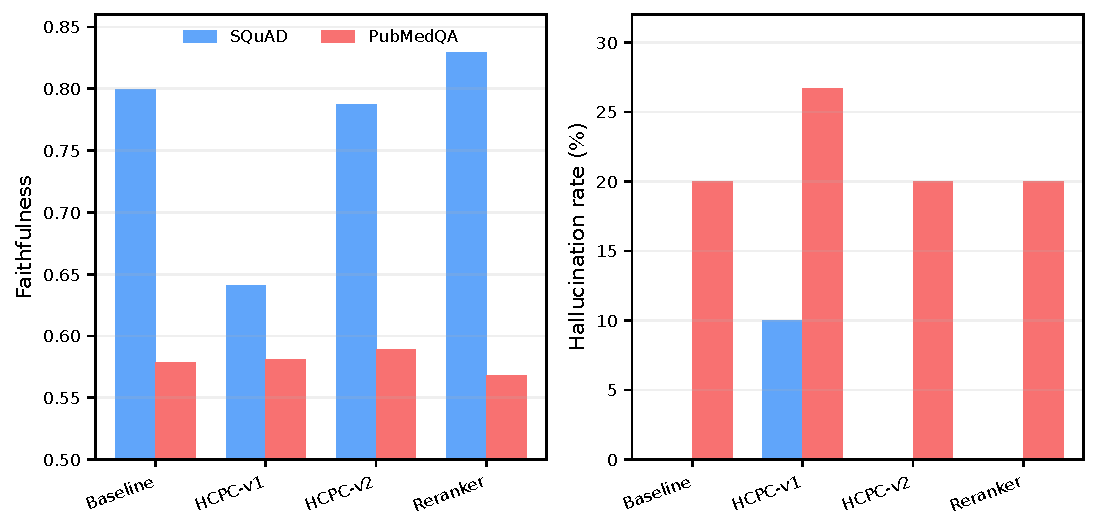
\includegraphics[width=\linewidth]{retrieval_comparison.pdf}
  \caption{Retrieval strategy comparison across conditions and datasets. HCPC-v1 degrades SQuAD faithfulness while HCPC-v2 recovers near-baseline performance.}
  \label{fig:retrieval_comparison}
\end{subfigure}
\hfill
\begin{subfigure}[t]{0.48\linewidth}
  \centering
  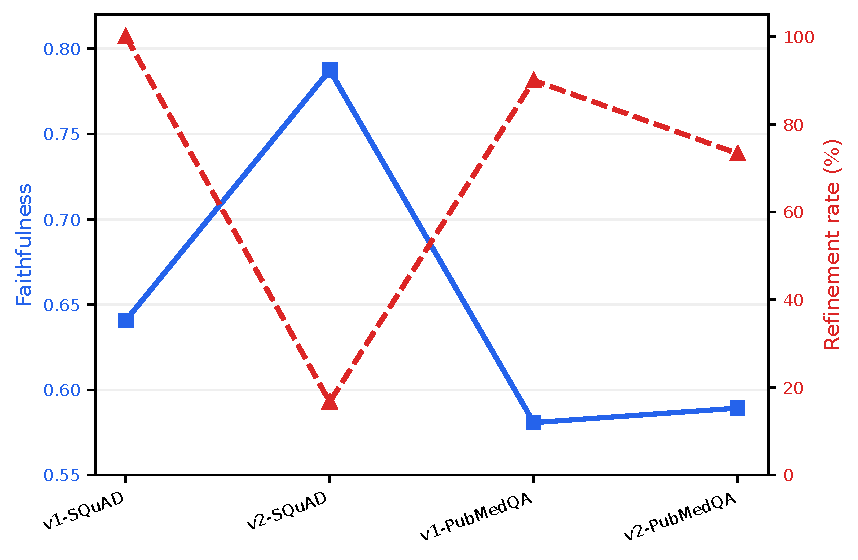
\includegraphics[width=\linewidth]{refinement_tradeoff.pdf}
  \caption{Faithfulness versus refinement rate. The largest quality gain appears exactly where HCPC-v2 suppresses unnecessary refinement.}
  \label{fig:refinement_tradeoff}
\end{subfigure}
\caption{Selective refinement recovers faithfulness through restraint. (a)~Across retrieval conditions, HCPC-v2 matches baseline faithfulness on SQuAD by avoiding the over-intervention that causes HCPC-v1 to fail. (b)~The recovery is tightly coupled to the reduction in refinement rate, supporting the claim that over-intervention is the primary source of degradation on domain-matched corpora.}
\label{fig:retrieval_tradeoff_combined}
\end{figure}
